\begin{figure}[p]
\centering
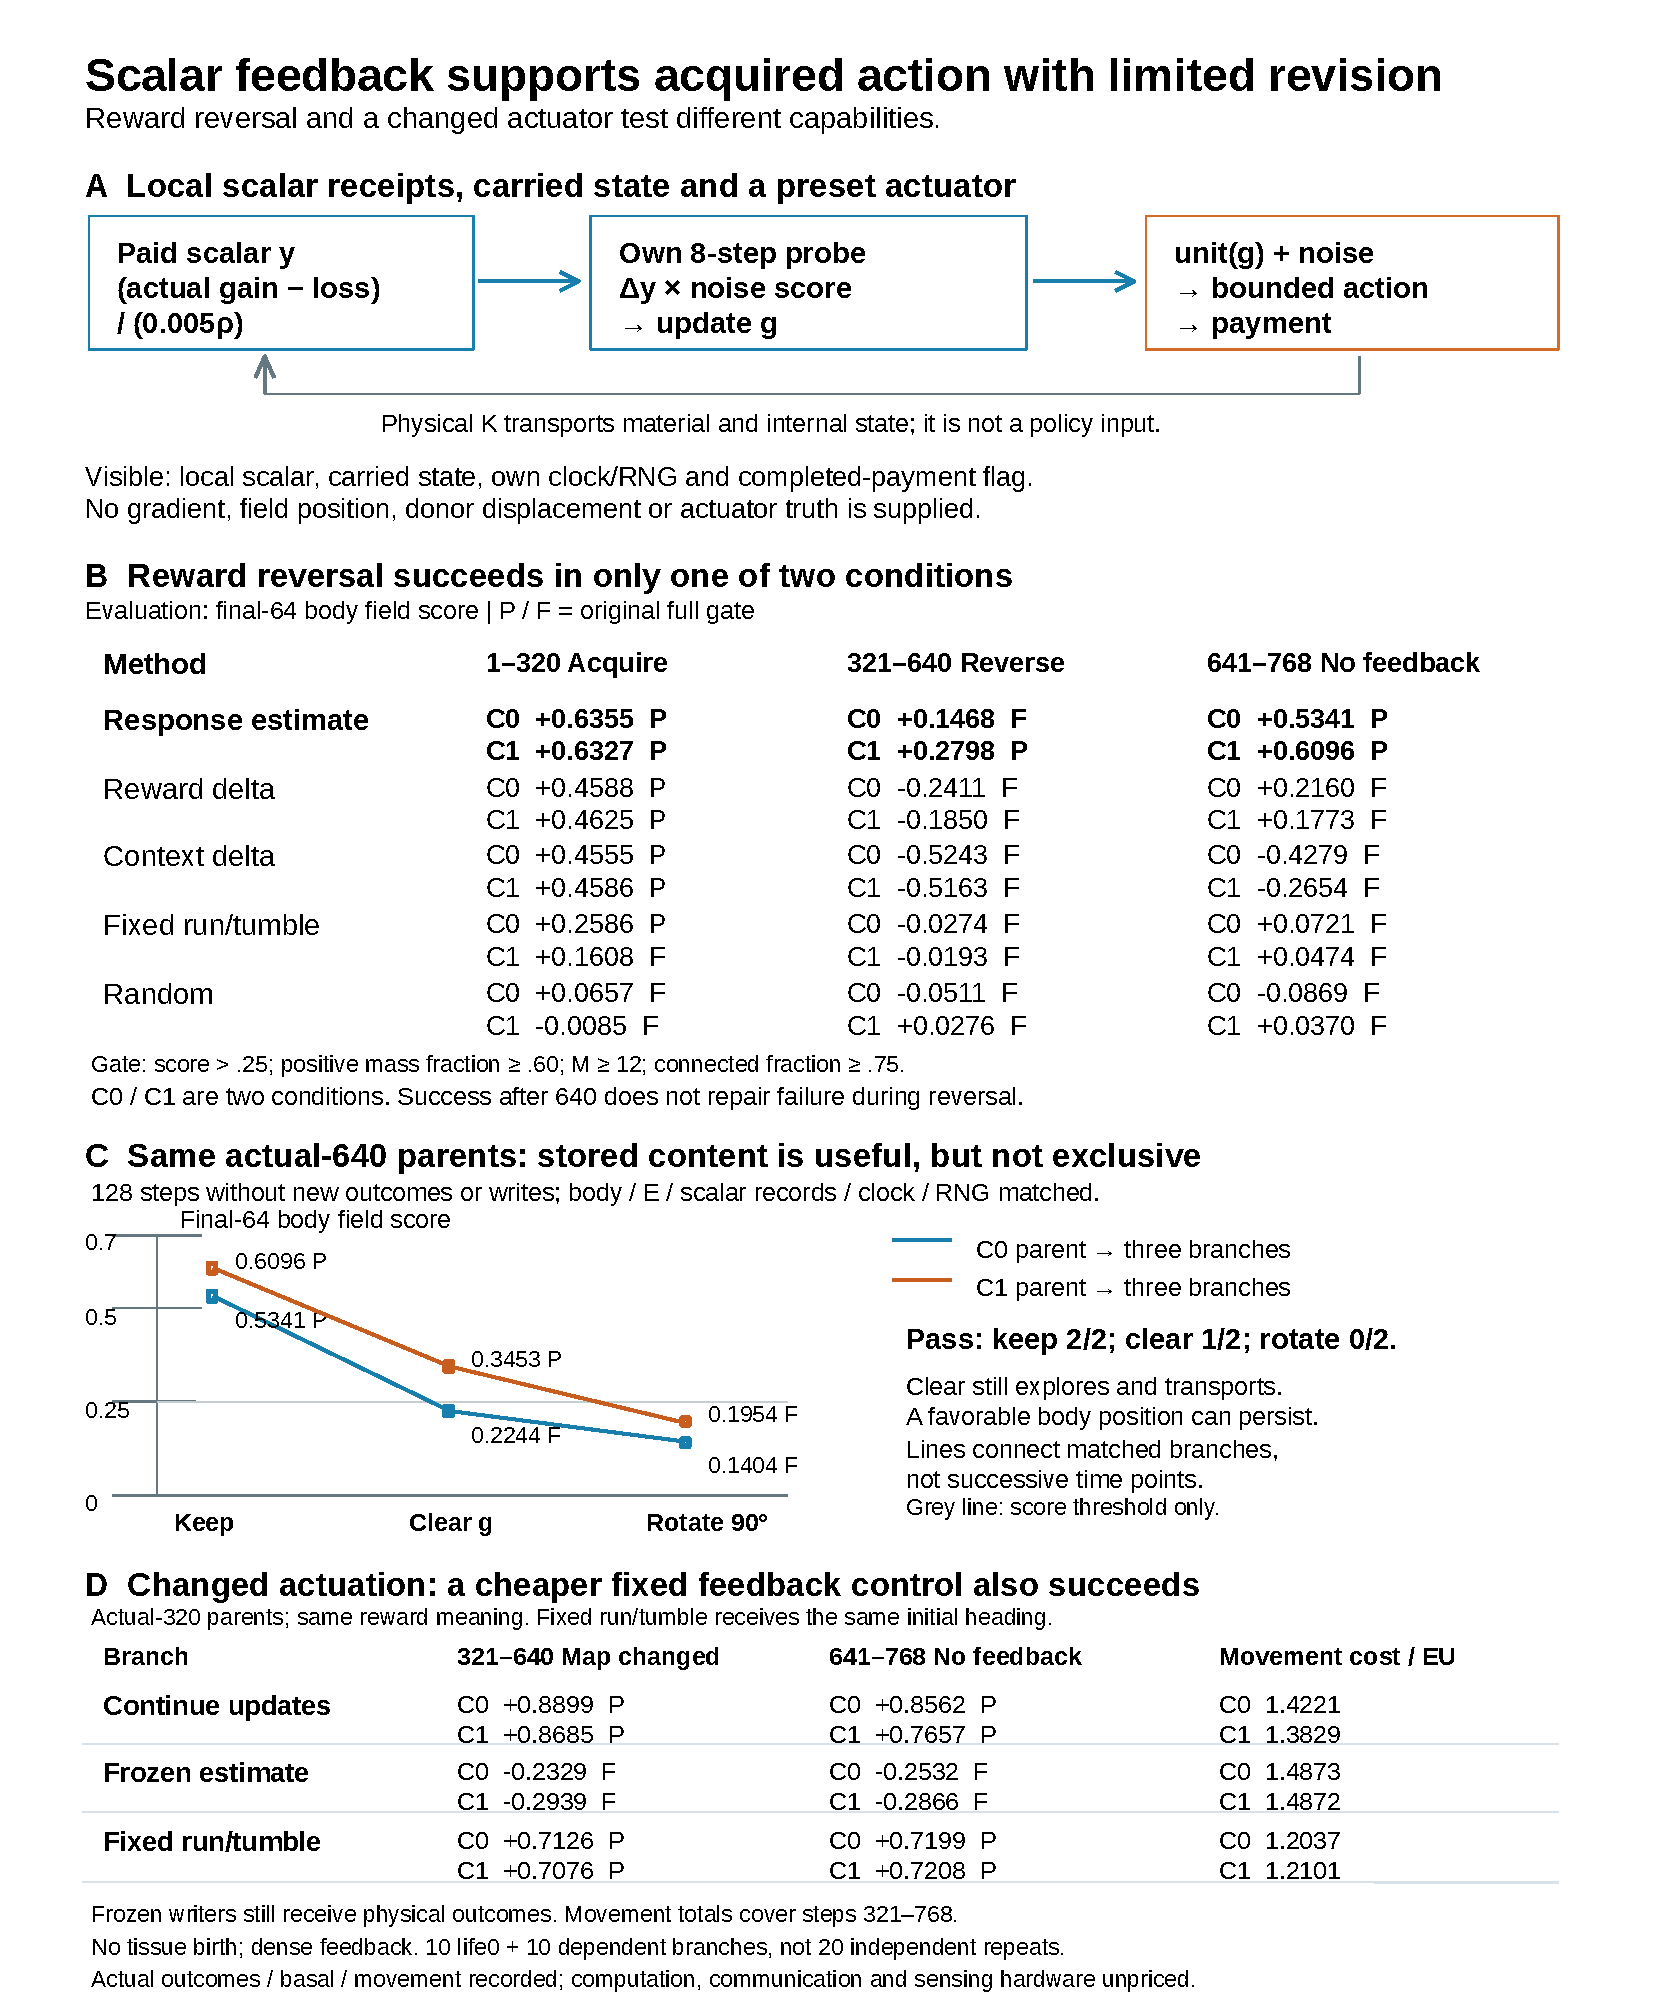
\includegraphics[width=\linewidth,height=0.68\textheight,keepaspectratio]{work/longform_v047/figures/scalar_action_v048/scalar_action.pdf}
\captionsetup{font=footnotesize}
\caption{\textbf{Scalar-only experience supports action acquisition, with different limits under reward and execution changes.}
\textbf{a}, A standard local response estimate uses completed scalar outcome changes and physically carried perturbation records. The transport operator $K$ moves material and internal state but provides no learner-facing displacement, gradient, field coordinate or actuator truth. Motion axes, cohesion, exploration and energy measurement are supplied.
\textbf{b}, All five methods, two paired seed--actuator conditions and three phases. Cells give final-64 mass-weighted field scores and the original complete gate (P/F); these evaluation quantities are not policy inputs. Response estimation passes acquisition in both conditions, reward reversal in one and the following no-new-feedback interval in both. The later success does not revise the failed reversal.
\textbf{c}, Two actual step-640 parents with response retained, cleared or rotated. Lines join related content interventions, not successive times. Retention passes twice, clearing once and rotation never. Clear branches still explore and move; rotation preserves response norm but not each bounded command or expense. Retained tails reuse recorded trajectories without replay.
\textbf{d}, From actual step-320 parents, only the physical execution map changes. Continued estimation and fixed run/tumble both pass the paid and later no-new-feedback windows in both conditions; frozen estimation fails. The fixed control receives the same acquired initial heading and spends less on movement. Expenditure sums both continuation phases. Ten new life-zero paths and ten dependent branches are not twenty independent repetitions. The conservative host has no tissue birth; physical expense is reported without a separate tariff for computation or sensing hardware. All phase outcomes and accounts are retained in the accompanying scalar-action source tables.}
\label{fig:scalar-action}
\end{figure}
